\chapter{Architektur und Realisierung}
Im folgenden Abschnitt wird die Architektur der Applikation diskutiert. Die Architektur ist so gewählt, dass die einzelnen funktionalen Komponenten zueinander eine tiefe Abhängigkeit aufweisen und dadurch eine weitere Entwicklung möglichst einfach ist.

\section{Struktur der Applikation}
%ja, plural ist Status, http://de.wikipedia.org/wiki/Status
Die Applikation hat im Grunde zwei Status, einerseits werden vor dem Rennen die Fahrerliste und die Marschtabelle importiert, andererseits wird die Rennsituation während dem Rennen erfasst und Änderungen festgehalten. Diese beiden Status können aber nicht absolut voneinander getrennt werden, da während dem Rennen Änderungen denkbar sind. Während dem Rennen müssen gewisse Daten immer angezeigt werden. Diese Live Informationen werden deshalb als eigene Ebene abgebildet. Aus den Anforderungen und den Kriterien entsteht folgende baumartige Struktur.

\begin{figure}[h!]
\caption{Struktur der Applikation als Organigramm}
\centering
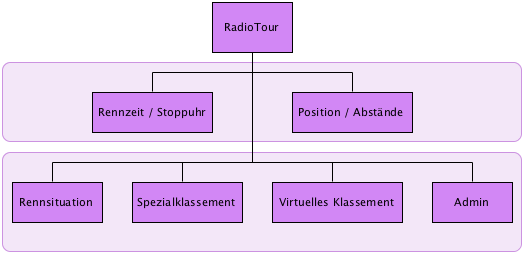
\includegraphics{05bericht/images/struktur.png}
\end{figure} 

Der Stamm stellt die Applikation dar und die Äste zeigen die Aufteilung der Funktionen. Die Rennzeit sowie die aktuelle Rennposition sind in einem immer sichtbaren Bereich platziert.
\\
Die untere Ebene beinhaltet die Kernelemente der Applikation. Diese werden in Views seitenweise dargestellt. Durch eine Navigation lässt sich zwischen den Views wechseln, ohne dass dabei die Live Informationen ausgeblendet werden.


\section{Klassendiagramm}
Die Domainlogik beinhaltet die Kernelemente der Applikation. Einerseits sind dies die Rennfahrer, welche Informationen über sich festhalten, andererseits die Etappe mit den Informationen zur Strecke. Während dem Rennen werden die Fahrer in Gruppen unterteilt. Auch diese Gruppen sind in der Domain abgebildet. Das Klassendiagramm des Domain Package zeigt die wesentlichen Elemente.

\begin{figure}[h!]
\caption{Die Domainklassen in der Abhängigkeit}
\label{fig:domain}
\centering
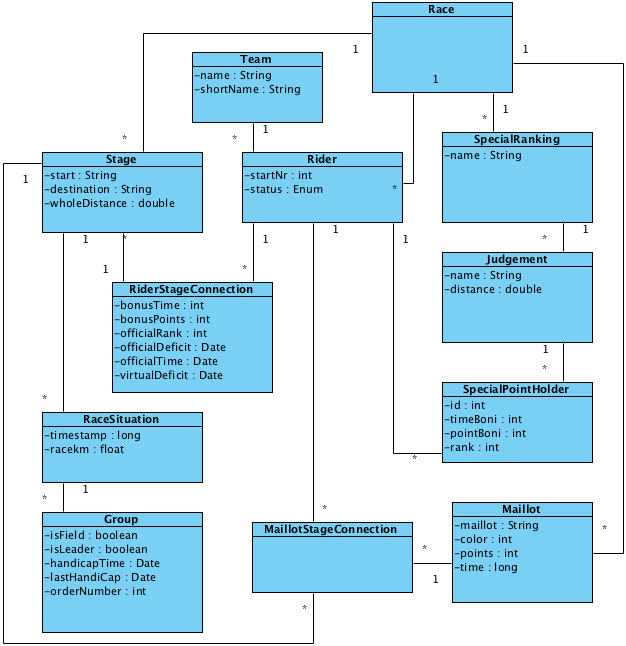
\includegraphics[scale=0.9]{05bericht/images/domain.png}
\end{figure} 


Die Klasse \textit{Rider} speichert die Angaben zu einem Fahrer und beinhaltet keine eigene Logik. Objekte dieser Klasse dienen als Stammdaten für alle Etappen welche in der Applikation erfasst sind.
In \textit{Stage} ist die Etappe definiert. Jede Etappe hat eine Marschtabelle in Form von mehreren \textit{PointOfRace} Objekten. Diese Objekte werden durch Import der Marschtabelle erstellt.
\\

Da pro Etappe jeder \textit{Rider} einen anderen \textit{RiderState} haben kann, gibt es die Verbindungsklasse \textit{RiderStageConnection}. In dieser Klasse ist jeweils die Etappe mit dem Fahrer verknüpft. Dies ermöglicht es, den Rückstand eines Fahrers in mehreren Etappen differenziert zu verfolgen. Dadurch werden bei einem Etappenwechsel innerhalb der Applikation immer die Informationen zur ausgewählten Etappe verwendet.

Die Klasse \textit{SpecialRanking} stellt ein Spezialklassement dar und wird benötigt, damit die einzelnen Wertungen (\textit{Judgement}), welche Etappenbasiert sind auch über alle Etappen hinweg zu verrechnen.

Eine \textit{RaceSituation} stellt einen Stand von \textit{Group} Objekten zu einem speziellen Zeitpunkt und Kilometerstand dar.

\section{Sequenz Diagramm}
Der häufigste UseCase besteht darin, die Rennsituation zu erfassen und an den Server zu übermitteln. Gleichzeitig werden im Hintergrund die Live Informationen aktualisiert. Diese beiden Hauptanwendungsfälle sind im folgenden System Sequenz Diagramm dargestellt. Der Actor wird durch den \textit{RadioTour Speaker} dargestellt und das System durch die \textit{RadioTour} Applikation. Das externe System stellt die Serverseite dar.

\begin{figure}[h!]
\caption{Das System Sequenz Diagramm}
\label{fig:ssd_rennen}
\centering
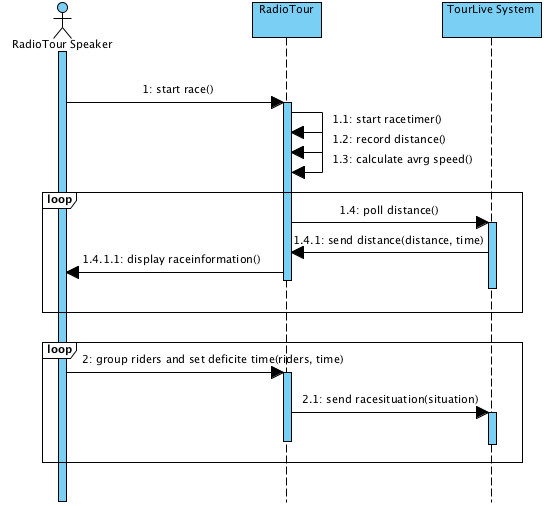
\includegraphics{05bericht/images/ssd_rennen.png}
\end{figure} 

Das Rennen wird durch das Starten der Rennzeit gestartet. Ab diesem Zeitpunkt beginnt die Aufzeichnung des Rennkilometers und die Berechnung der durchschnittlichen Geschwindigkeit.


\section{Realisierung}
Lorem ipsum dolor sit amet, consetetur sadipscing elitr, sed diam nonumy eirmod tempor invidunt ut labore et dolore magna aliquyam erat, sed diam voluptua. At vero eos et accusam et justo duo dolores et ea rebum. Stet clita kasd gubergren, no sea takimata sanctus est Lorem ipsum dolor sit amet. Lorem ipsum dolor sit amet, consetetur sadipscing elitr, sed diam nonumy eirmod tempor invidunt ut labore et dolore magna aliquyam erat, sed diam voluptua. At vero eos et accusam et justo duo dolores et ea rebum. Stet clita kasd gubergren, no sea takimata sanctus est Lorem ipsum dolor sit amet.